\documentclass{article}

\usepackage{arxiv}

\usepackage[utf8]{inputenc} % allow utf-8 input
\usepackage[T1]{fontenc}    % use 8-bit T1 fonts
\usepackage{hyperref}       % hyperlinks
%\usepackage{url}            % simple URL typesetting
%\usepackage{booktabs}       % professional-quality tables
\usepackage{amsfonts}       % blackboard math symbols
%\usepackage{nicefrac}       % compact symbols for 1/2, etc.
%\usepackage{microtype}      % microtypography
%\usepackage{lipsum}
%\usepackage{fancyhdr}       % header
\usepackage{graphicx}       % graphics
\usepackage{verbatim} 
\usepackage{amsmath}

\graphicspath{{./images/}}

  
%% Title
\title{Equipotential curves on water surface}

\author{
  Kirill A. Smirnov, Dmitriy V. Spinov \\
  Letovo School \\
  Moscow\\
  \texttt{spinov.d@phystech.edu} \\
  \texttt{smirnov4kirill@yandex.ru} \\
}


\begin{document}
\maketitle


\begin{abstract}
	
\end{abstract}


\section{Introduction}            %%%%%%%%%%%%%%%%%            
An electric field arises in the space surrounding an electric charge. The electric field exerts an electric force. The potential at a point in the electric field is the work done in bringing a unit positive charge from infinity to the given point. If charge distribution does not change over time, the potential of the points is constant. An equipotential curve is a curve on which the potential is the same over the curve. The displacement of a charge over such a curve would require no work.\par

Some studies on the subject have already been done. The basis of the subject is long-known Gauss' law \cite{gauss}, \cite{landavshic}. In "An experiment on equipotential curves"\cite{khaparde} potential around different-shaped electrodes was experimentally explored. Also, a formula for the case of cylindrical coaxial electrodes was derived theoretically. The problem of potential produced by static charges on cylindrical coaxial electrodes was explored in "A Simple Electric Field Probe in a Gauss's Law Laboratory"\cite{ludwigsen} and "Electrostatic field plotting apparatus" \cite{smith}. The case of conductive paper as the medium was also considered in "Equipotential Surfaces of Various Charge Configurations" \cite{beyond}.

The automation of line-measurement developed in "High-density electric potential plots" \cite{binder2015high}.

We have researched the subject in the condition of two small cylindrical electrodes, placed on opposite sides of the measuring area. We used an electrolytic tank with water of different salinities as conducting medium.


%\section{Experimental Setup}

\begin{figure}[h]
	\begin{center}
		\begin{minipage}[h]{0.47\linewidth}
			\center{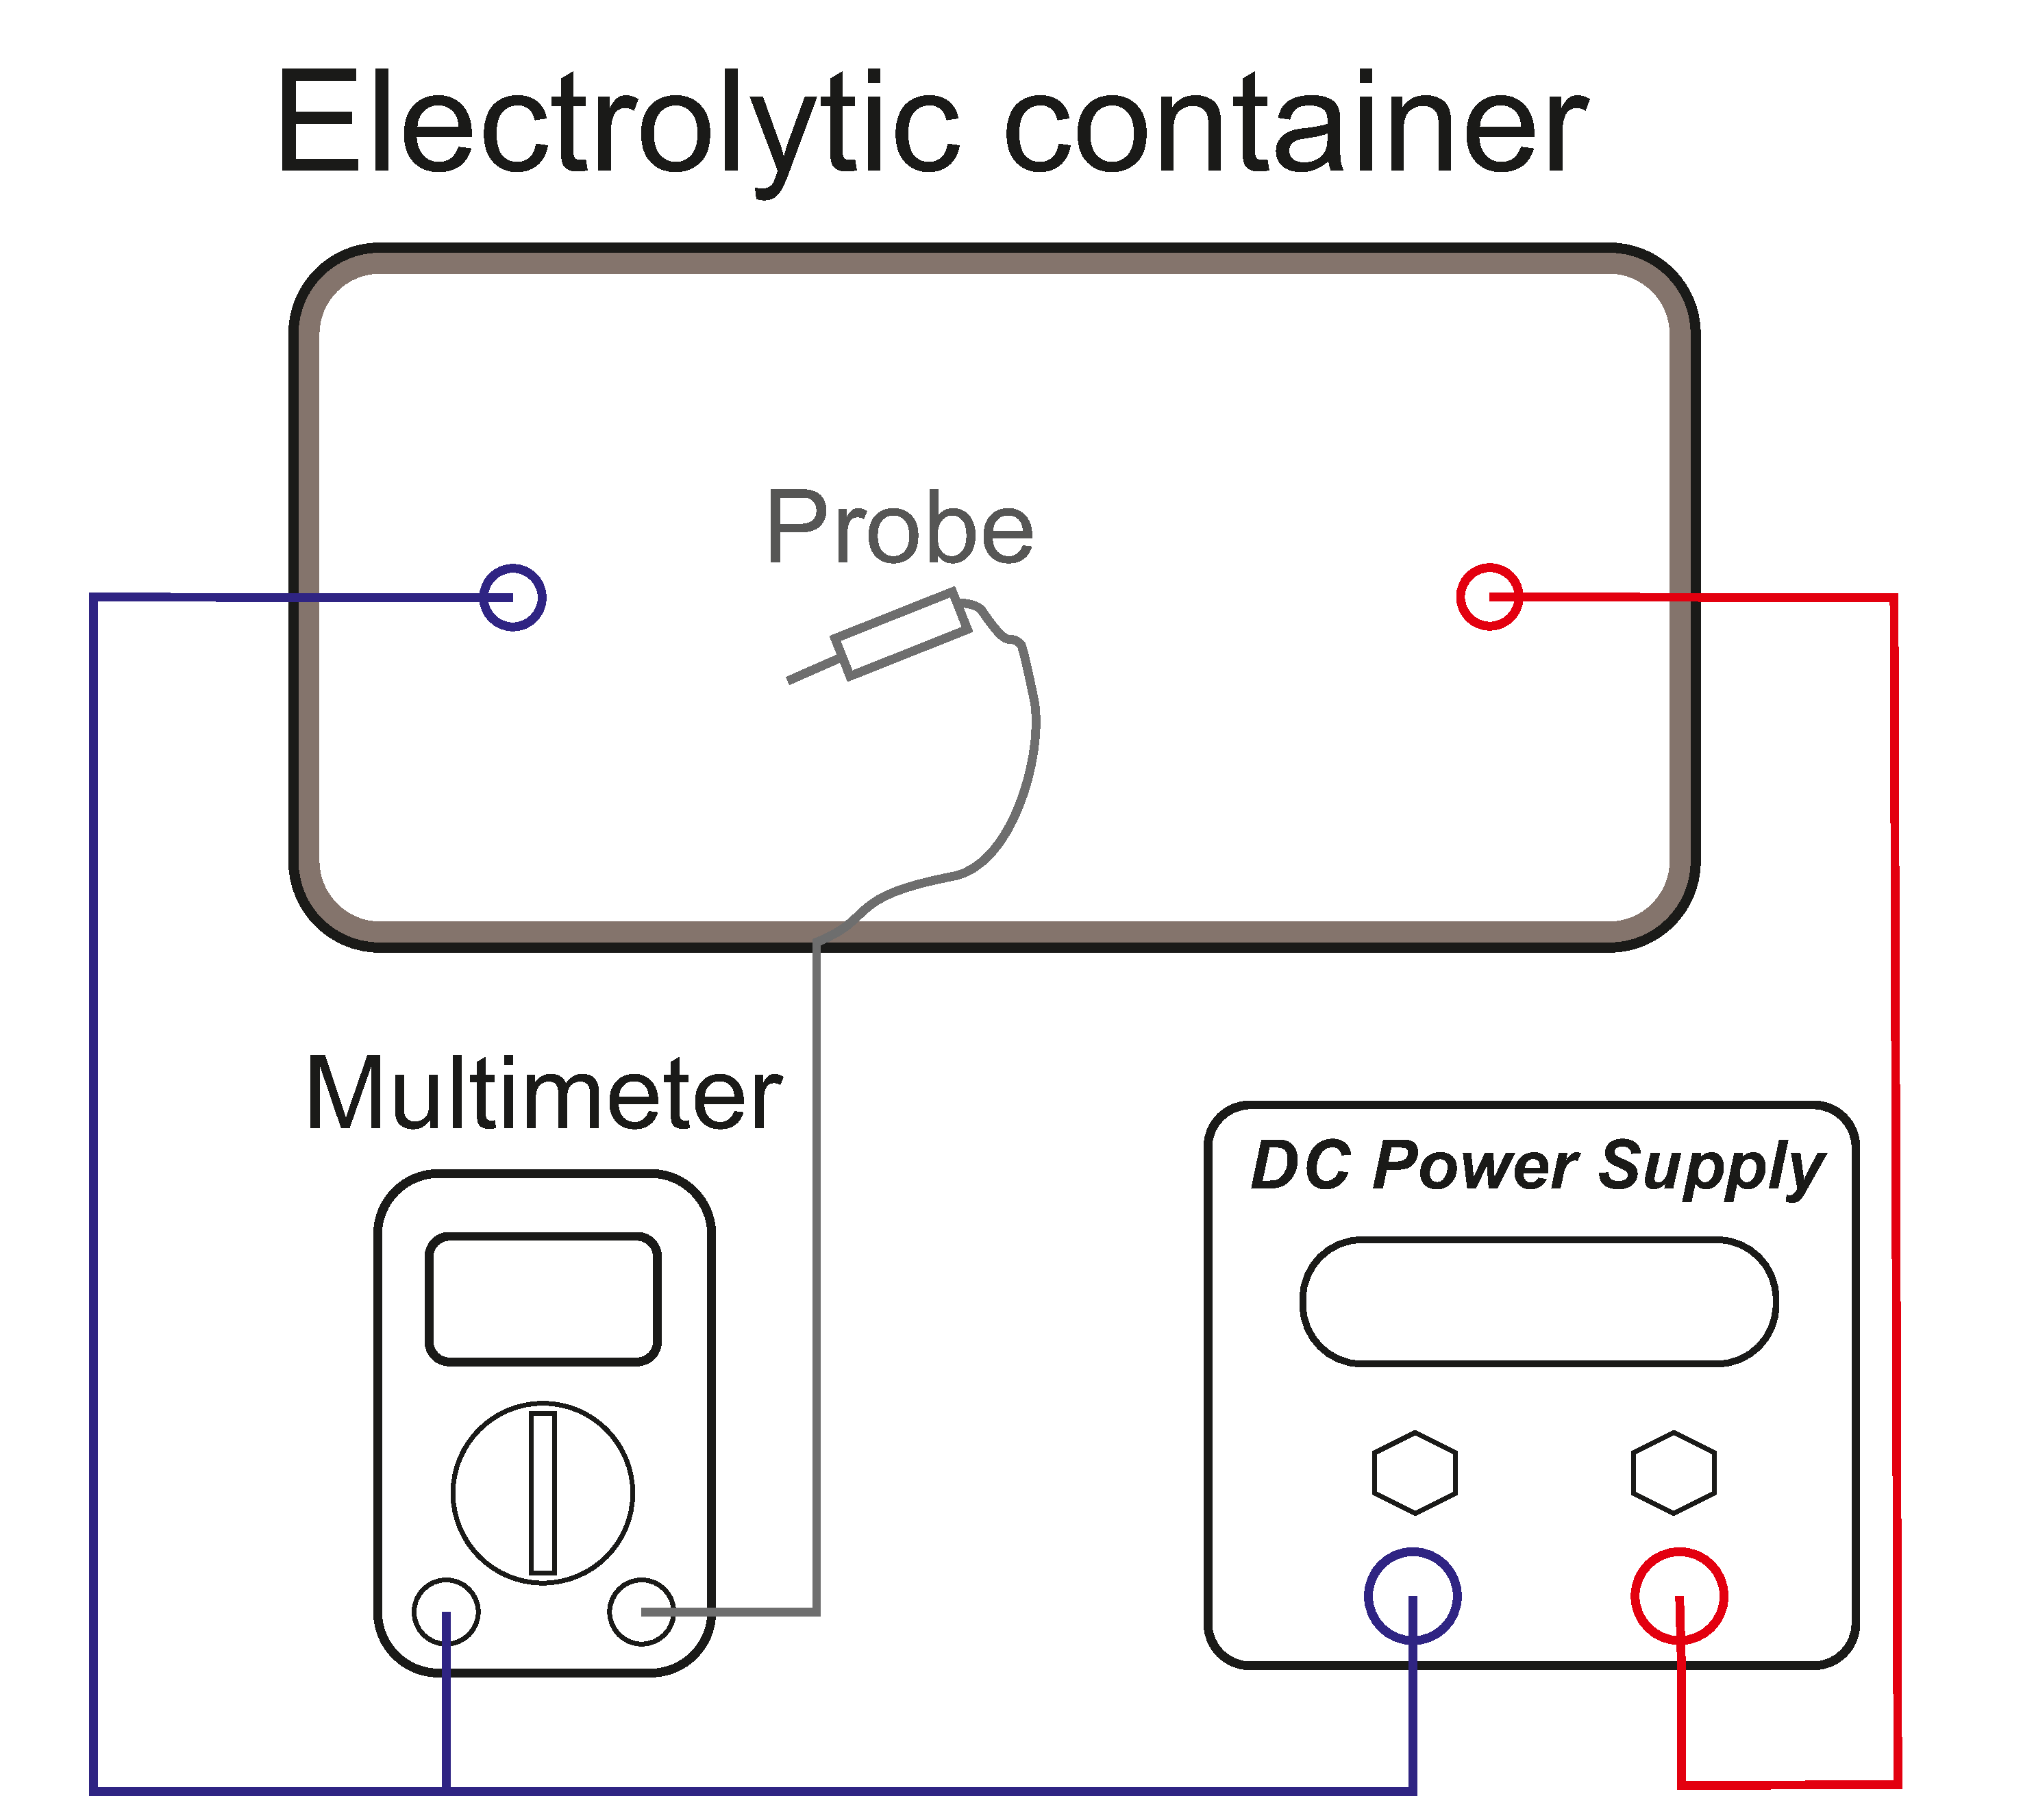
\includegraphics[width=1\linewidth]{scheme1.pdf}}
			\caption{Scheme of the manual experiment setup}
			\label{fig:mesh1}
		\end{minipage}
		\hfill
		\begin{minipage}[h]{0.47\linewidth}
			\center{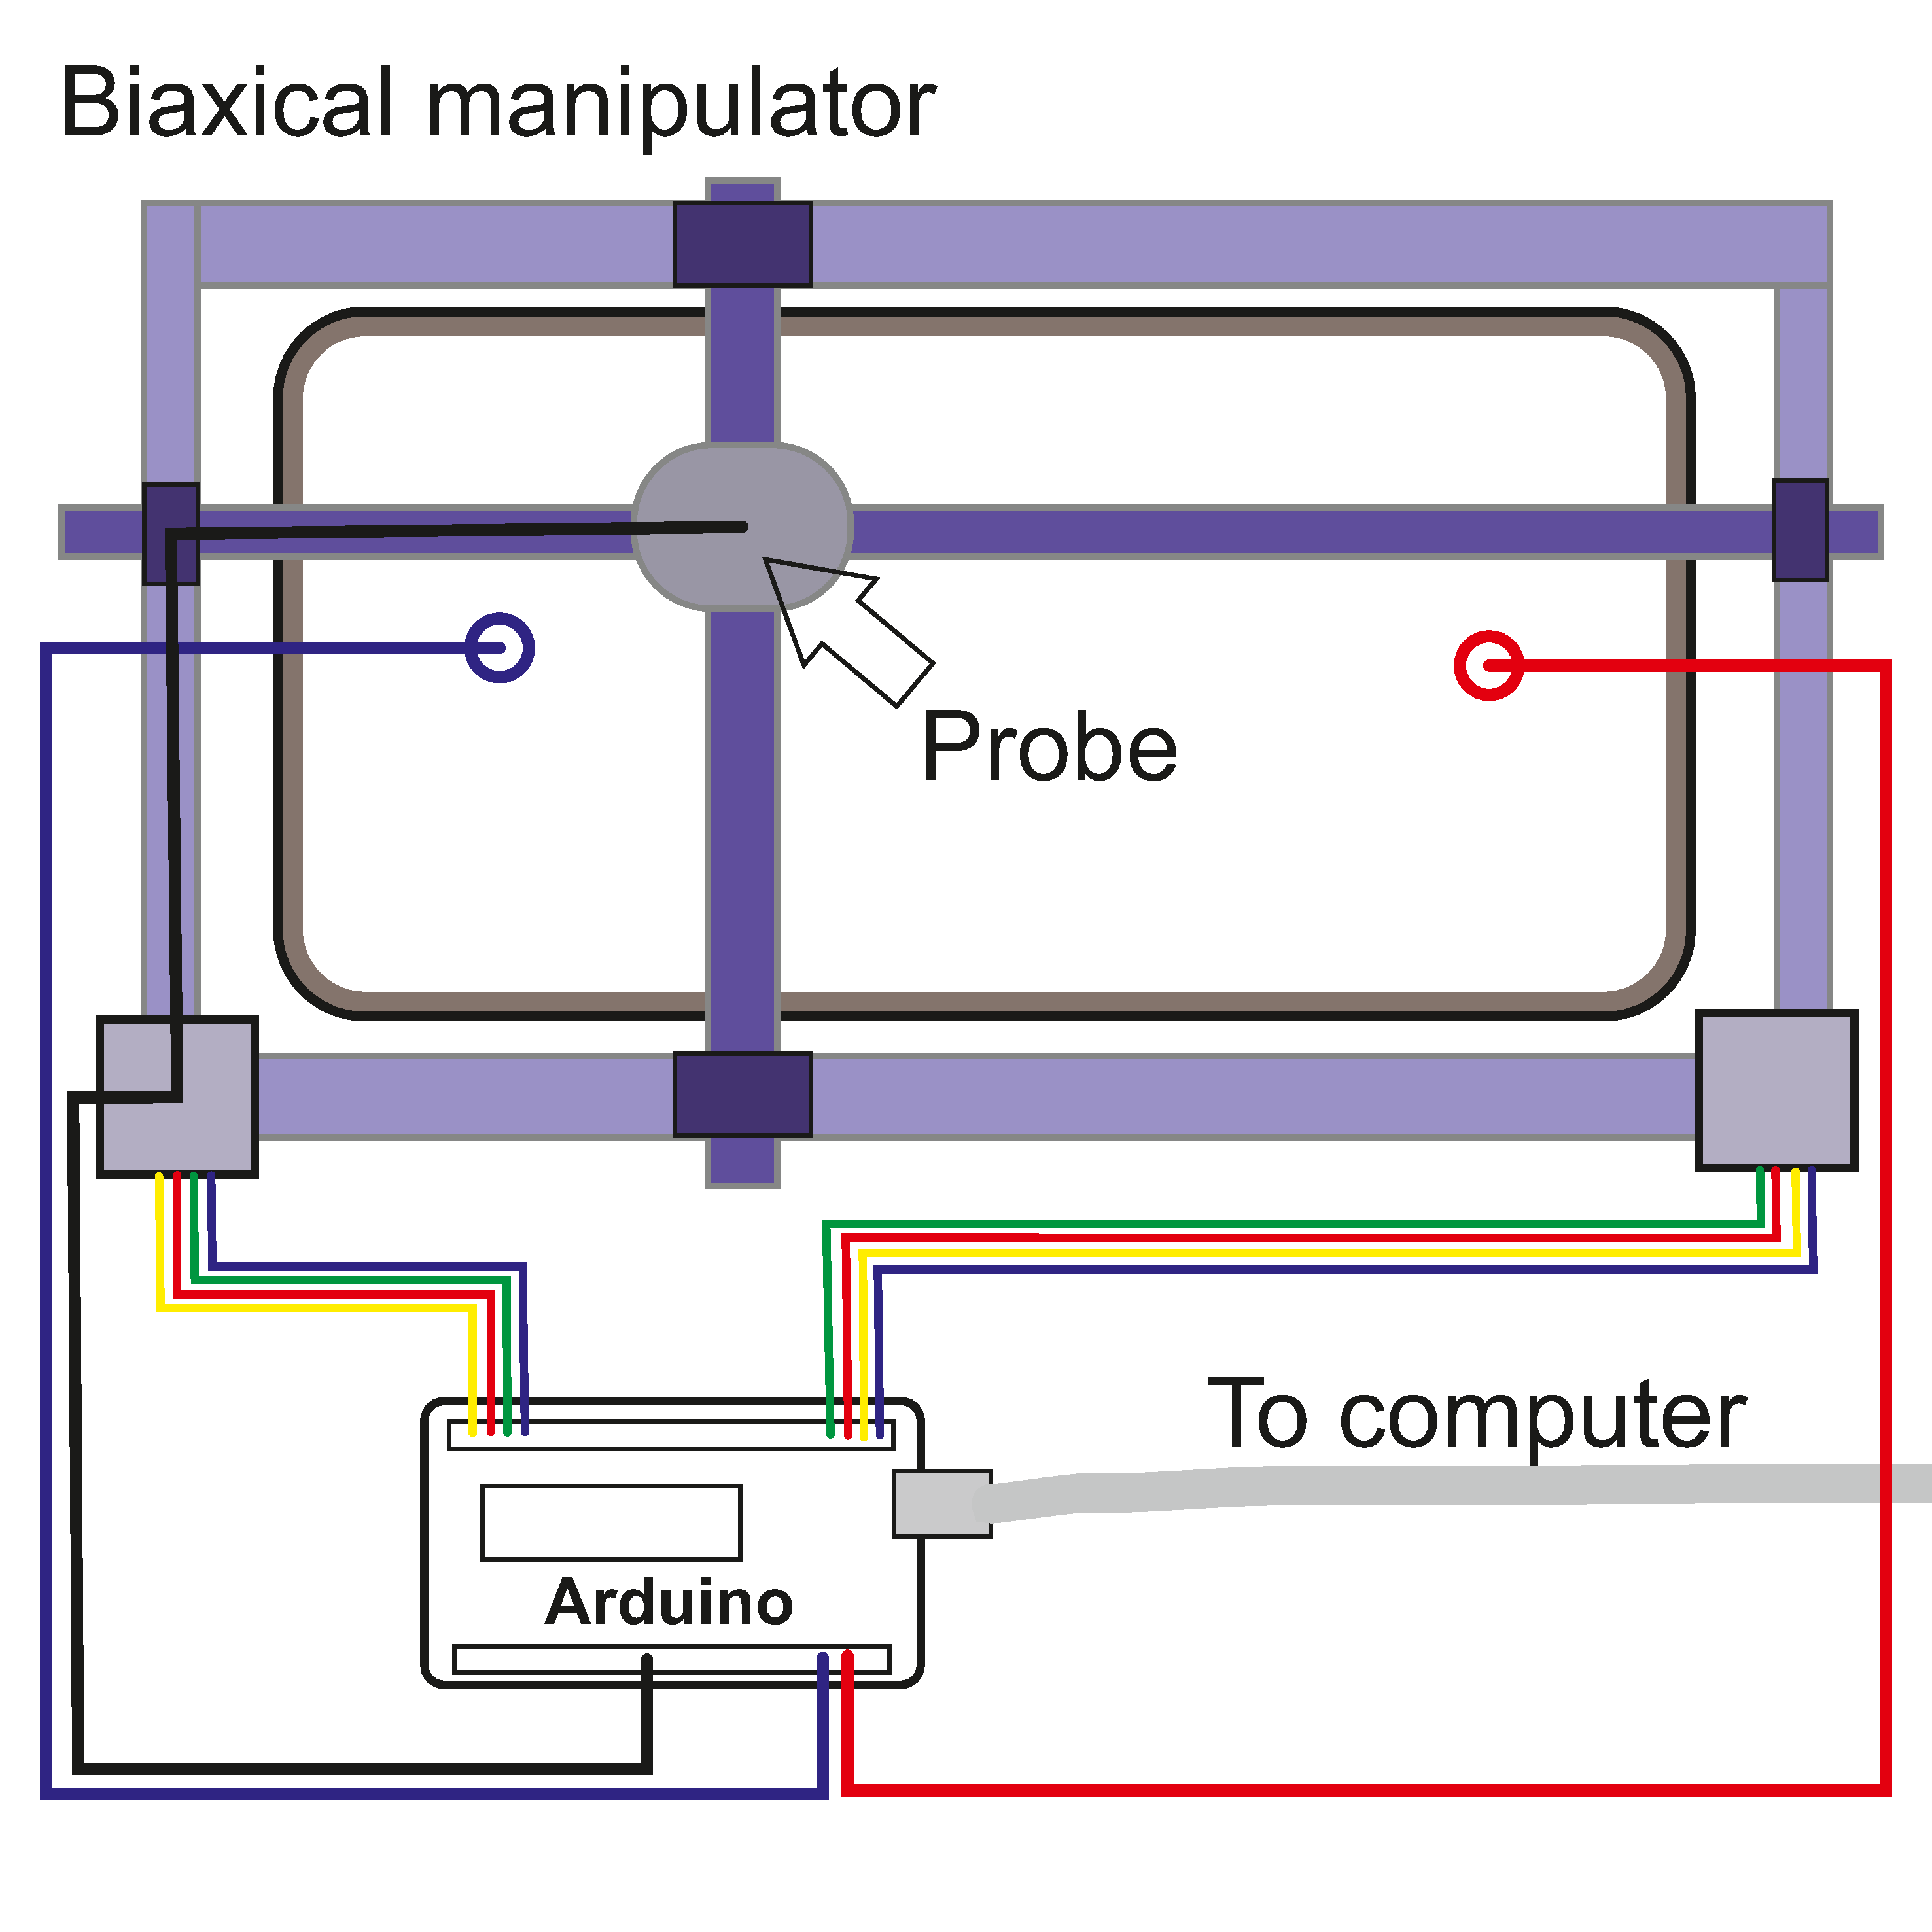
\includegraphics[width=1\linewidth]{scheme2.pdf}}
			\caption{Scheme of the experiment using the biaxical manipulator}
			\label{fig:mesh2}
		\end{minipage}
	\end{center}
\end{figure}


\begin{figure}[h]
	\begin{center}
		\includegraphics[width=0.75\linewidth]{20220209_143045.jpg}
		\caption{Photo of the manipulator}
		\label{manipulator_photo}
	\end{center}
\end{figure}



For the simplest experimental setup are needed the following materials: a container with electrolyte (distilled water), a DC power supply with two electrodes, and a voltmeter. Put the electrodes in the water, turn on the power, and measure the voltage with a voltmeter. Also, a non-conductive checkered sheet can be put in the water to know the coordinates of the point you are measuring. Scheme is in the figure \ref{fig:mesh1}.  \par

For making a significant amount of experiments this method is time-consuming, so we robotized the measuring process. We used a biaxial manipulator, that can move the voltmeter probe and write the measure value and coordinates of the probe to a file on a computer. The manipulator has a 383 x 367 mm work zone with an accuracy of 0.1 mm. It contains 2 42BYG stepper motors and a MegaPi motor driver. We used Arduino Uno as a control board.


In both experimental setups, we used \textbf{non-conductive container} to eliminate the possibility of current flowing through the walls.\par

It is important to control the substances dissolved in water, so we used distilled water solution with $Na_2SO_4$ because sodium sulfate does not oxidize electrodes, except for sodium chloride, which we used at first. Electrode oxidizing is harmful because it changes the composition of the water, which can affect the voltage of the electrolyte.\par

As we observed, potentials are not time-independent certain time after applying voltage. The voltage difference between electrodes and the near electrolyte is increasing from 0 to a fixed amount (what causes voltage drop near electrodes), so we waited for 1 minute until the potentials get stabilized. The same effect is observed with the probe, so the probe is needed to move slowly (about 5 mm per second). More about the phenomenon later. \par


\section{Theory}

To describe current in a continuum we can use Gauss's law \cite{gauss}, \cite{landavshic} 
\begin{equation}
  \begin{aligned}
  \nabla\cdot E (x, y) = \frac{\rho (x, y)}{\varepsilon_0 \varepsilon_r}
  \end{aligned}
\end{equation}
	  
   which represents the relations between electric field and charge density at any point. \par

\begin{figure}[h]
    \centering
    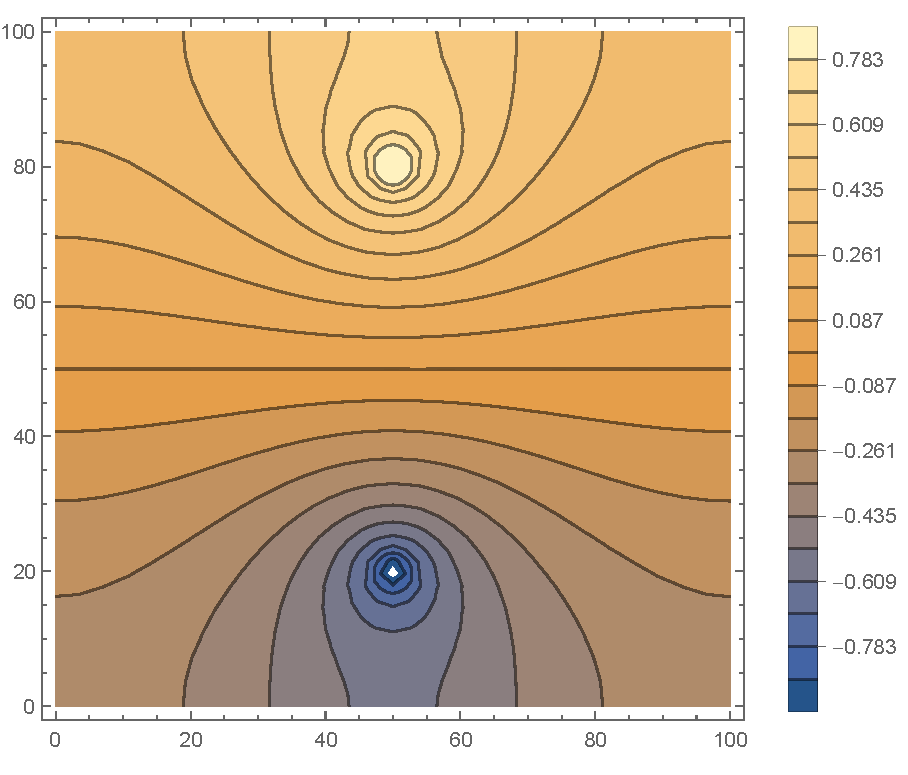
\includegraphics[width=0.5\textwidth]{theory plot.pdf}
    \caption{Voltage plot}
    \label{fig:mesh3}
\end{figure}

We assumed that away from the electrodes water is electrically neutral, which can be verified with an electroscope, so
\begin{equation}
  \begin{aligned}
    \rho (x, y) = 0 \Rightarrow\\
  	\nabla \cdot E (x, y) = 0 \Rightarrow \\
    \Delta \varphi (x, y) = 0 
  \end{aligned}
\end{equation}
what is a Laplacian equation, which can be solved knowing boundary conditions:
\begin{equation}
  \begin{aligned}
    \varphi (x, y) = -1 V, (x - x_1)^2 + (y - y_1)^2 = r_1^2 \\
    \varphi (x, y) = +1 V, (x - x_2)^2 + (y - y_2)^2 = r_2^2
  \end{aligned}
\end{equation}

where $x_1, y_1, r_1, x_2, y_2, r_2$ are coordinates and radii of two circle electrodes. The equation can be solved using Wolfram Mathematica. The plot is in the figure \ref{fig:mesh3}. \par



\section{Observations and Experimental results}

%%%%%%%%%%%%%%%%%%%%%%%%%%%%%%%%%%
\begin{figure}[htb!]
\begin{center}
\begin{minipage}[h]{0.47\linewidth}
\center{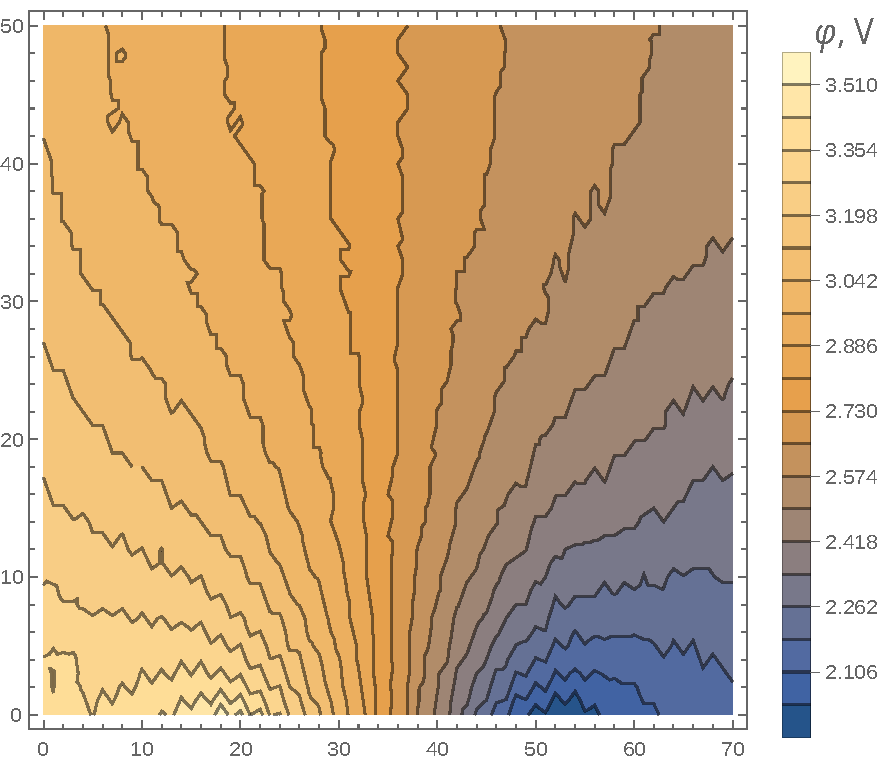
\includegraphics[width=1\linewidth]{8.8 d raw.pdf}}
%\caption{Photo of the experiment setup} %% подпись к рисунку
%\label{fig:mesh1} %% метка рисунка для ссылки на него
\end{minipage}
\hfill
\begin{minipage}[h]{0.47\linewidth}
\center{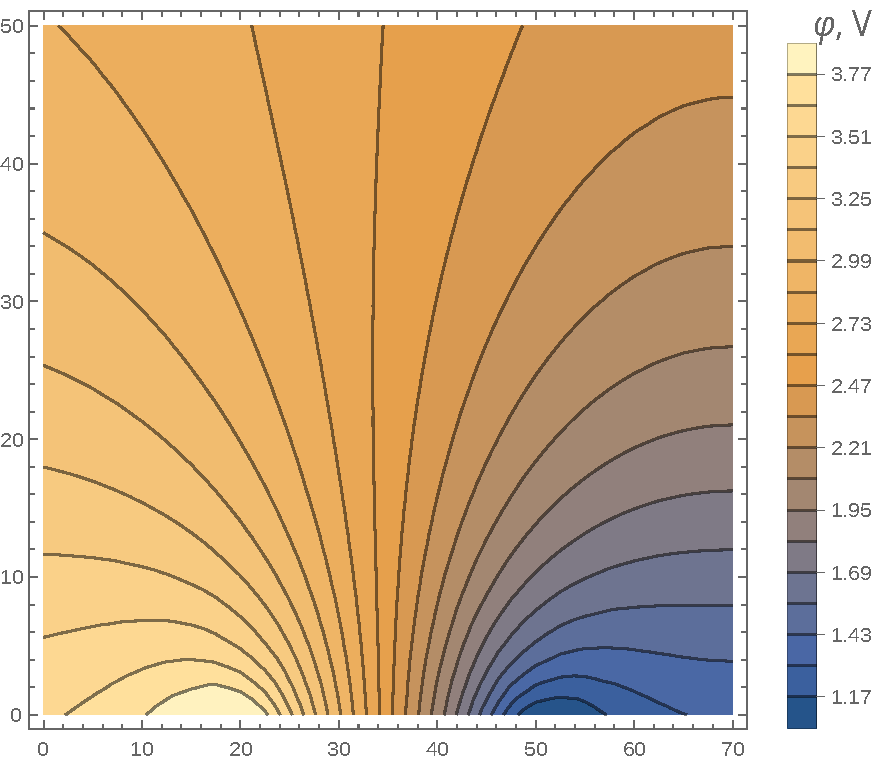
\includegraphics[width=1\linewidth]{vert theory.pdf}}
%\caption{Photo of the biaxical manipulator} %% подпись к рисунку
%\label{fig:mesh2} %% метка рисунка для ссылки на него
\end{minipage}


\caption{Comparison of theoretical prediction and experiment data for 8.8 grams to 1 kg of water}
\label{fig:mesh4}

%\vfill

%\end{center}
\end{center}
\end{figure}
\begin{figure}
\begin{center}

\begin{minipage}[h]{0.47\linewidth}
\center{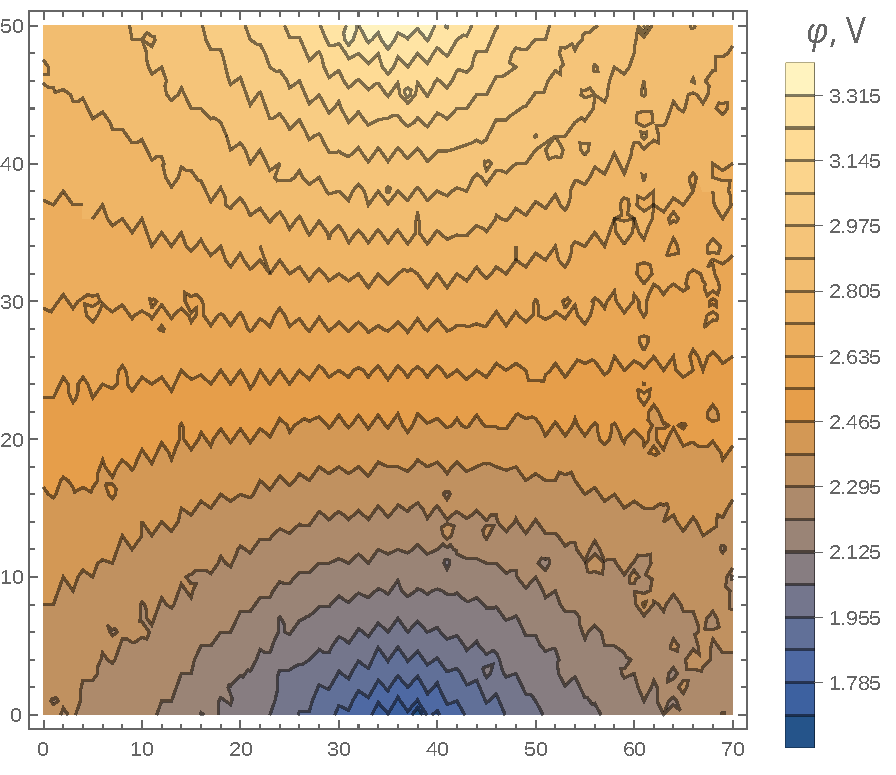
\includegraphics[width=1\linewidth]{2.3 g raw.pdf}}
%\caption{Photo of the experiment setup} %% подпись к рисунку
%\label{fig:mesh1} %% метка рисунка для ссылки на него
\end{minipage}
\hfill
\begin{minipage}[h]{0.47\linewidth}
\center{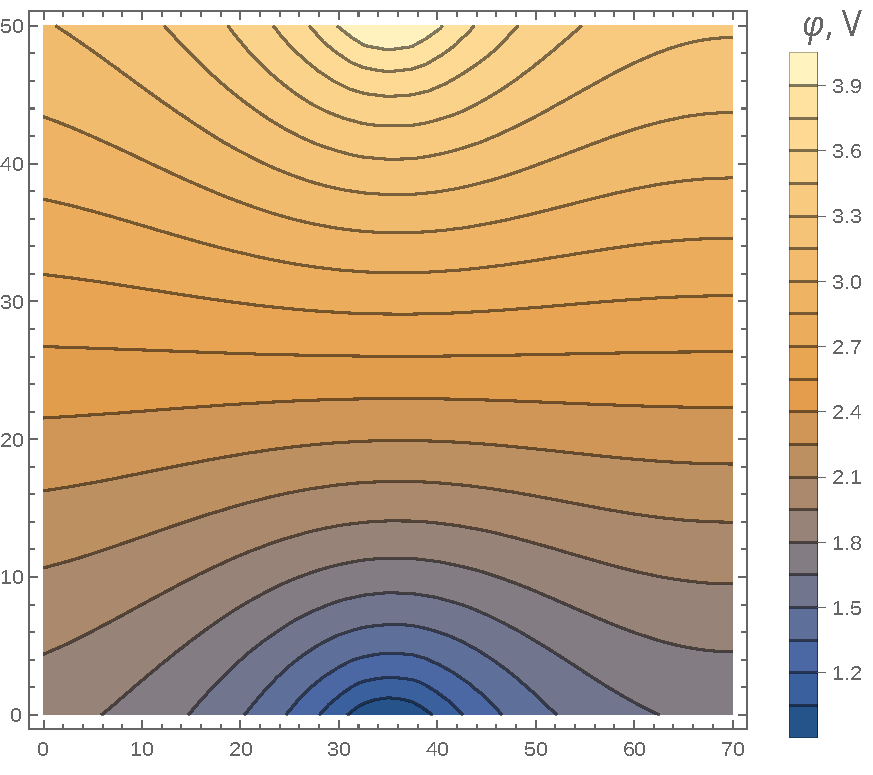
\includegraphics[width=1\linewidth]{hor theory.pdf}}
%\caption{Photo of the biaxical manipulator} %% подпись к рисунку
%\label{fig:mesh2} %% метка рисунка для ссылки на него
\end{minipage}
\caption{Comparison of theoretical prediction and experiment data for 2.3 grams to 1 kg of water}
\label{fig:mesh5}

%\vfill
\end{center}
\end{figure}
\begin{figure}
\begin{center}

\begin{minipage}[h]{0.47\linewidth}
\center{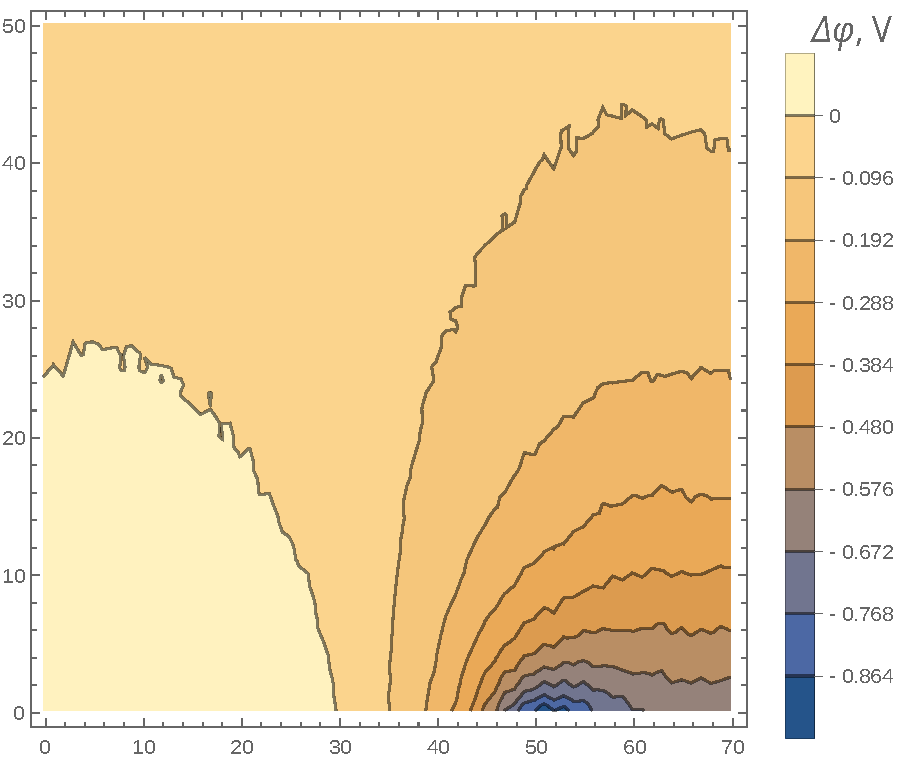
\includegraphics[width=1\linewidth]{difSol6Norm.pdf}}
\caption{Normed error of figure \ref{fig:mesh4} experiment}
\label{fig:dif6}
\end{minipage}
\hfill
\begin{minipage}[h]{0.47\linewidth}
\center{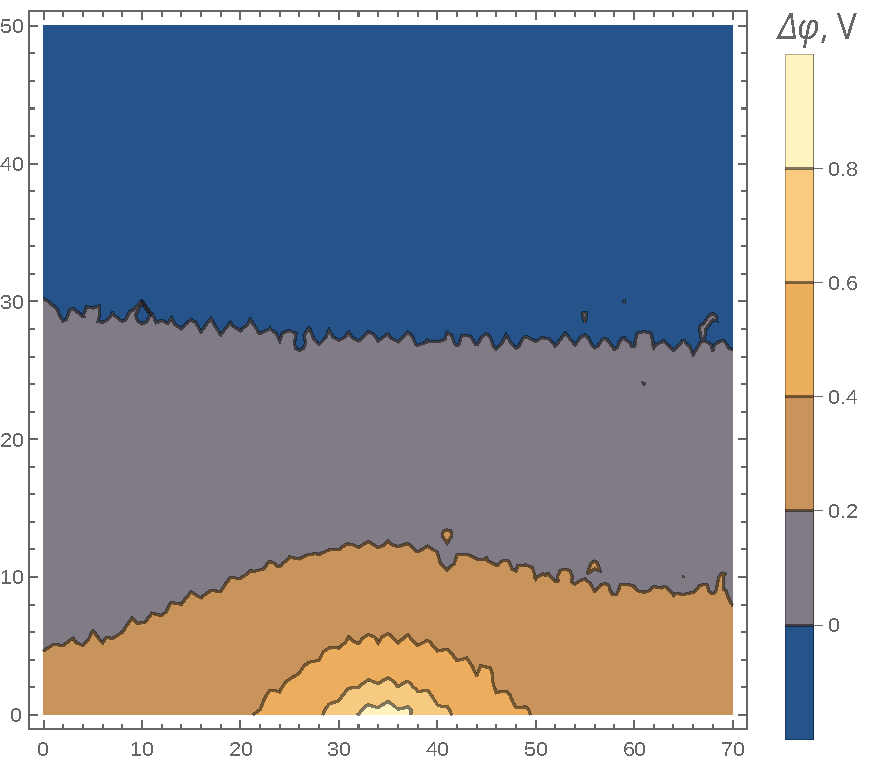
\includegraphics[width=1\linewidth]{difSol2Norm.pdf}}
\caption{Normed error of figure \ref{fig:mesh5} experiment}
\label{fig:dif2}
\end{minipage}


\end{center}
\end{figure}
%%%%%%%%%%%%%%%%%%%%%%%%%%%%%%%%%%%%5

\begin{figure}[htb!]
\begin{center}
\begin{minipage}[h]{0.47\linewidth}
\center{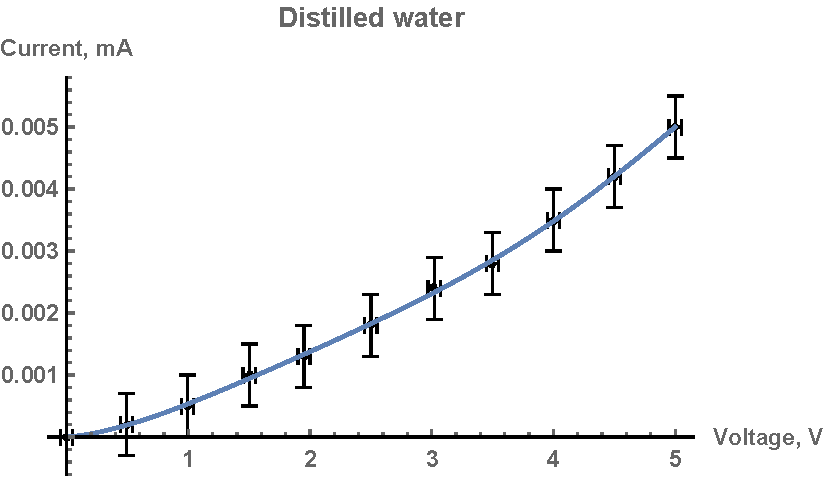
\includegraphics[width=0.9\linewidth]{distilled VAC.pdf}}
%\caption{Photo of the experiment setup} %% подпись к рисунку
%\label{fig:mesh1} %% метка рисунка для ссылки на него
\end{minipage}
\hfill
\begin{minipage}[h]{0.47\linewidth}
\center{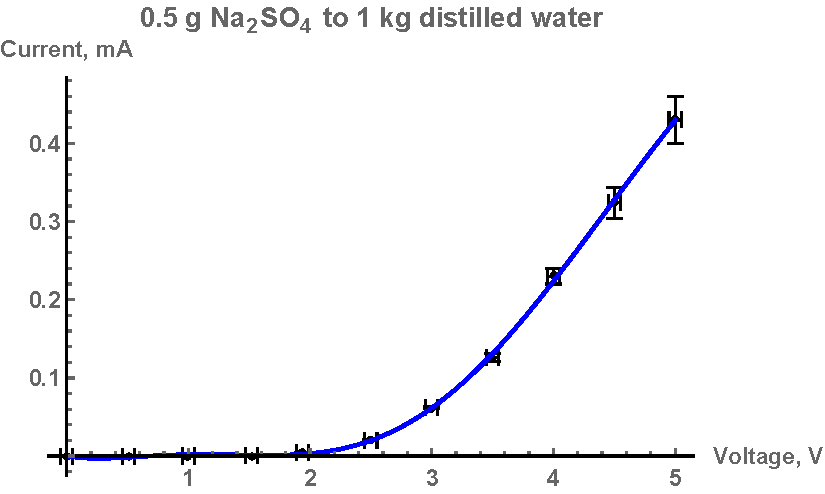
\includegraphics[width=0.9\linewidth]{0.5g.pdf}}
%\caption{Photo of the biaxical manipulator} %% подпись к рисунку
%\label{fig:mesh2} %% метка рисунка для ссылки на него
\end{minipage}
\end{center}

\caption{Electrical Characteristics}
\label{fig:VACs}
\end{figure}

\begin{figure}[htb!]
\begin{center}
\center{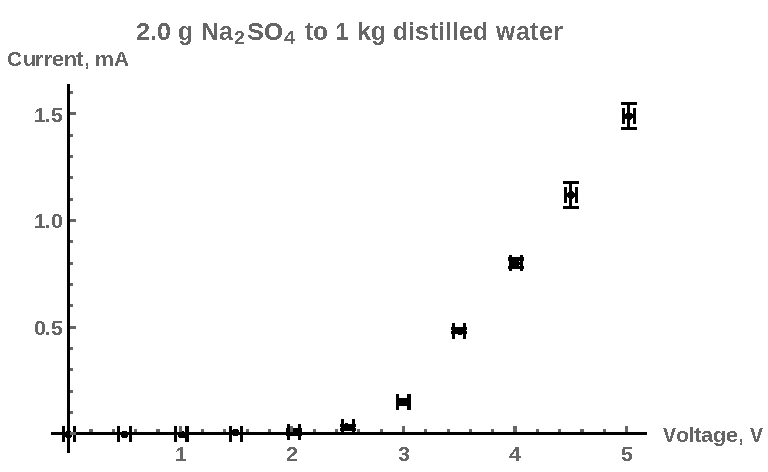
\includegraphics[width=0.7\linewidth]{2.0_g_VAC2.pdf}}
\end{center}
\caption{Characteristic for considering}
\label{fig:VAC}
\end{figure}

Raw data and code for the manipulator can be found at \url{https://github.com/Kirill4Smirnov/Equipotentials}. \par

Experimental and theoretical plots are in the figures \ref{fig:mesh4} and \ref{fig:mesh5}. The error of the experiments is about 0.05 V. Measurement of the voltmeter resistance is difficult, because we used Arduino as a voltmeter, and it applies a voltage to the sensor pin if the current through the pin is small (about 5 mA). \par


As we can see in the figures \ref{fig:mesh4}, \ref{fig:mesh5}, \ref{fig:dif6} and \ref{fig:dif2}, the theory can quite accurate predict the shape of the equipotential curves, but gives too big error in prediction a specific potential (the shape of the curves also is consistent with the measurements of paper \cite{binder2015high}). \textbf{The max error is about 80 \% near electrodes.} From surface science we know about the phenomenon named double electric layer \cite{kinetika}, \cite{stillinger}. The phenomenon causes voltage drop near electrodes, so the potential in the electrolyte around the electrodes is different from the electrode potential. But the theoretical model works on the assumption that we know potential near the electrodes. We assumed that the potential near an electrode approximately equals the potential on the electrode. But because of the voltage drop, it does not. \par


As we observed, if we apply 5V to the electrode, the voltage near it is about 3.5 - 4.0 V and depends on the water salinity. Also, voltage drop depends on the shape of electrodes and the time elapsed since applying a constant voltage. The effect of voltage drop collapses if the electrolyte gets in motion (perhaps, the double layer disintegrates from fluid movement). During the experiments, we waited 1 minute for the voltage drop to stabilize before starting the measurement (AC voltage has not been studied).\par

We measured the Electrical Characteristics of different solutions, two plots are in the figure \ref{fig:VACs}. The step of the voltage is 0.5V. Errors are about 0.05V for the voltage axis and 5\% for the current axis (current was measured in different modes, therefore the accuracy is proportional to measurement value).

Solution characteristics provided in the figure \ref{fig:VACs} are ordinary for all studied solutions: in consists of 3 parts, which are provided in the figure \ref{fig:VAC}. The only exception is distilled water, which characteristic is linear.


Characteristic analysis:
\begin{enumerate}   
\item The first segment: according to the electric layer explanation, the layers formed by free ions compensate for the potential difference between the electrodes, hence the effective potential difference is close to 0, and therefore current is close to 0.

\item On this segment is a transition to a linear section. The piece can be called "activation", and the "activation voltage" we measured is about 3V.

\item The third segment is a linear dependence. The electric layers are fully formed and no longer change. The solution in this segment can be represented as a series connection of a resistor and a battery, where electric layers are the battery and the neutral solution is the resistor. The resistance of the continuum of water depends on the salinity of the solution.
\end{enumerate}

As we observed, "activation voltage" depends on the shape and the nature of the coating of the electrodes. We used a medical needle 1 mm thick.



\section{Acknowledgments}
I would like to express my deepest thanks to Aleksei Cherkasov and Artem D. Sukhov for helping write the article. I would also like to thank Ivan Kolesnikov for assistance with theory and Pavel A. Kotin for providing the necessary conditions for the research.

\bibliographystyle{plain}
\bibliography{refs}


\end{document}